%---------------------------------------------------------------------  
    \section{Metodología}
    %------------------------------ SLIDE ---------------------------------------
    % Cambia el símbolo del itemize a un triángulo negro
    %\setbeamertemplate{itemize item}{\raisebox{0.2ex}{\scriptsize$\blacktriangleright$}}
    %\setbeamercolor{itemize item}{fg=red} % Cambia el color del triángulo a naranja

    %\begin{frame}{Metodología} % cada entorno frame es una diapositiva
        %\justifying % para justificar el texto, siempre al inicio de cada frame
        % Añade espacio para mover el bloque hacia arriba
        % Añade espacio para mover el bloque hacia arriba
        %\vspace*{-1.4cm} % Ajusta este valor según sea necesario

        %\begin{columns}
            %\begin{column}{0.7\textwidth} % Columna izquierda para la lista
                %\textcolor{blue}{\textbf{CORSIKA:}}
                %\begin{itemize}
                    %\item Simulación de chubascos de partículas.
                    %\item Escrito en el lenguaje de \textbf{FORTRAN}.
                    %\item Modelo de interacción hadrónica para alta energía:
                        %\begin{itemize}
                            %\item \textbf{QGSJET-II}.
                        %\end{itemize}
                    %\item Modelo de interacción hadrónica para baja energía:
                        %\begin{itemize}
                            %\item \textbf{FLUKA}.
                        %\end{itemize}
                %\end{itemize}
            %\end{column}

            %\begin{column}{0.2\textwidth} % Columna derecha para la imagen
                %\begin{figure}
                    %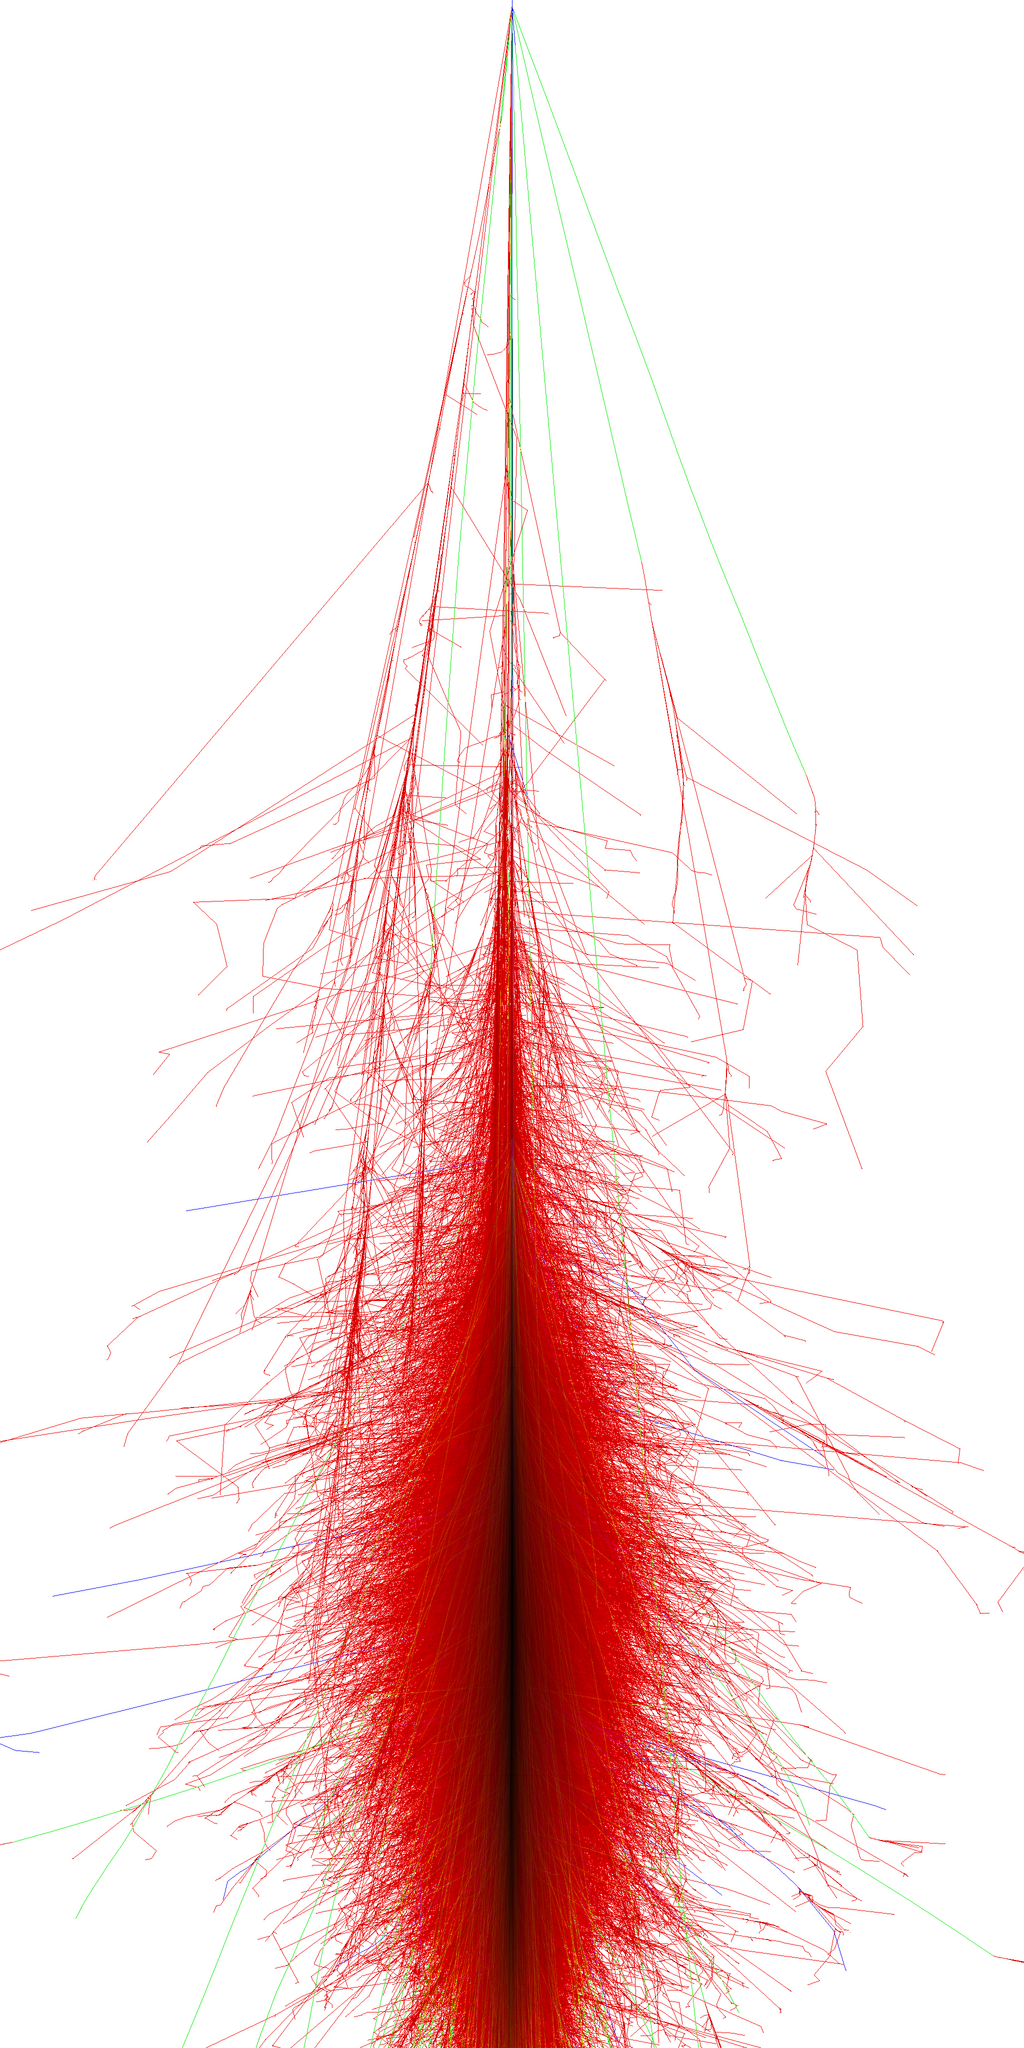
\includegraphics[width=0.7\textwidth]{Figures/corkisa-shower.png}
                    %\caption{\tiny Cascada de partículas producida por un protón, obtenida con \href{https://www-zeuthen.desy.de/~jknapp/fs/photon-showers.html}{CORSIKA} (2024).}
                %\end{figure}
            %\end{column}
        %\end{columns}
    %\end{frame} 

    %------------------------------ SLIDE ---------------------------------------
    \setbeamercolor{itemize item}{fg=orange} % Puedes cambiar el color del triángulo
    % Cambia el símbolo del itemize a un triángulo negro
    \setbeamertemplate{itemize item}{\raisebox{0.2ex}{\scriptsize$\blacktriangleright$}}
    \setbeamercolor{itemize item}{fg=red} % Cambia el color del triángulo a naranja

    \begin{frame}{Metodología} % cada entorno frame es una diapositiva
        \justifying % para justificar el texto, siempre al inicio de cada frame
        % Añade espacio para mover el bloque hacia arriba
        % Añade espacio para mover el bloque hacia arriba
        \vspace*{-0.3cm} % Ajusta este valor según sea necesario

        \begin{columns}
            \begin{column}{0.5\textwidth} % Columna izquierda para la lista
                \textcolor{blue}{\textbf{Ubicación geográfica de los puntos de observación:}}
                \begin{itemize}
                    \item Estudio in situ realizado por \cite{lara2016}.
                    \item Mediciones realizadas con el MNM portátil.
                    \item 41 puntos de observación.
                    \item Altitud más baja: $7$ m.s.n.m.
                    \item Altitud más alta: $4582$.5 m.s.n.m.
                \end{itemize}
            \end{column}

            \begin{column}{0.4\textwidth} % Columna derecha para la imagen
            \begin{figure}
                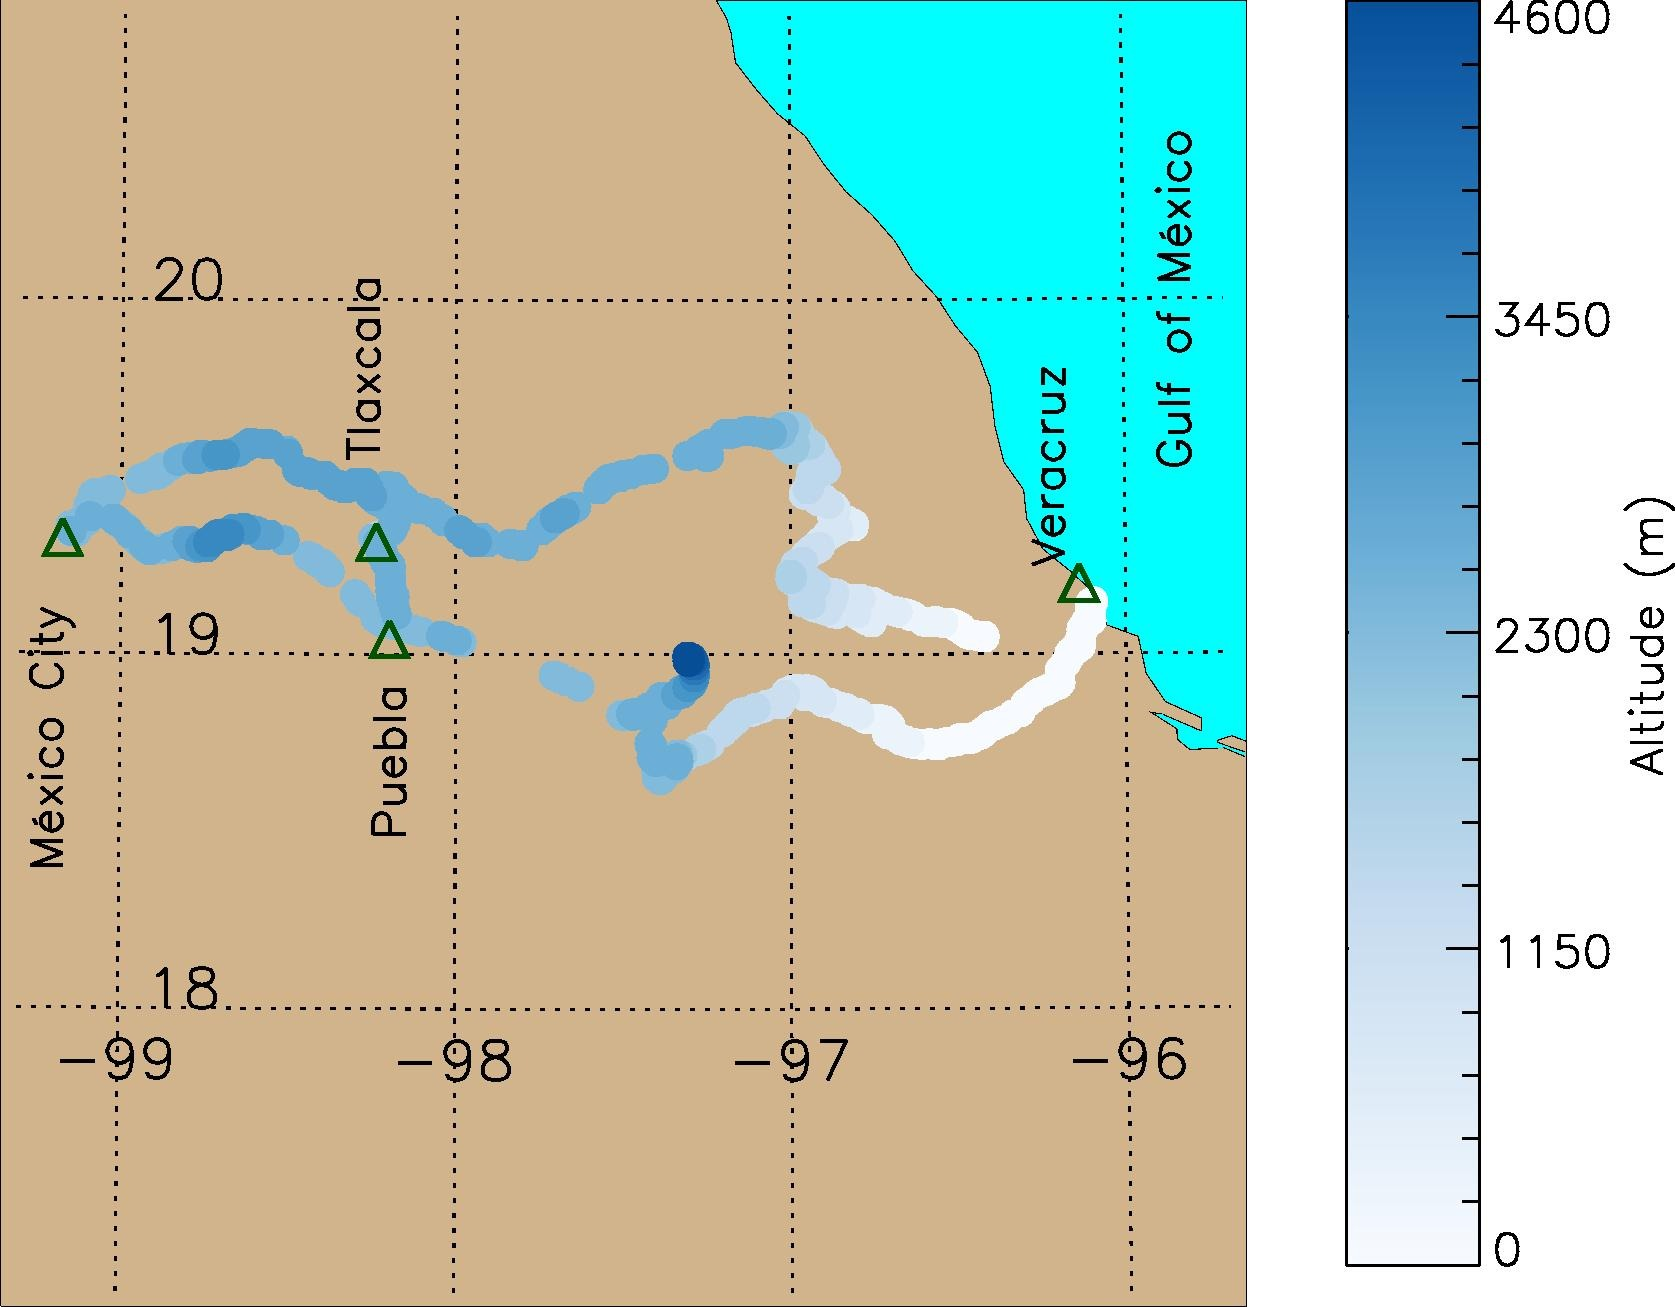
\includegraphics[width=1.1\textwidth]{Figures/map1.jpg}
                \caption{\tiny Mapa con los puntos donde [\cite{lara2016}] realizaron mediciones con su detector a diferentes altitudes. El color en los puntos va relacionado a la altitud. Los triángulos corresponden a las ciudades más pobladas.}
            \end{figure}
            \end{column}
        \end{columns}
    \end{frame}

    %------------------------------ SLIDE ---------------------------------------
    % Cambia el símbolo del itemize a un triángulo negro
    \setbeamertemplate{itemize item}{\raisebox{0.2ex}{\scriptsize$\blacktriangleright$}}
    \setbeamercolor{itemize item}{fg=red} % Cambia el color del triángulo a naranja

    \begin{frame}{} % cada entorno frame es una diapositiva
        \justifying % para justificar el texto, siempre al inicio de cada frame
        % Añade espacio para mover el bloque hacia arriba
        % Añade espacio para mover el bloque hacia arriba
        \vspace*{-0.1cm} % Ajusta este valor según sea necesario

        \begin{columns}
            \begin{column}{0.5\textwidth} % Columna izquierda para la lista
                \textcolor{blue}{\textbf{CORSIKA:}}
                \begin{itemize}
                    \item Simulación de chubascos de partículas.
                    \item Escrito en el lenguaje de \textbf{FORTRAN}.
                    \item Modelo de interacción hadrónica para alta energía:
                        \begin{itemize}
                            \item \textbf{QGSJET-II}.
                        \end{itemize}
                    \item Modelo de interacción hadrónica para baja energía:
                        \begin{itemize}
                            \item \textbf{FLUKA}.
                        \end{itemize}
                \end{itemize}
            \end{column}

            \begin{column}{0.4\textwidth} % Columna derecha para la imagen
                \begin{figure}
                    %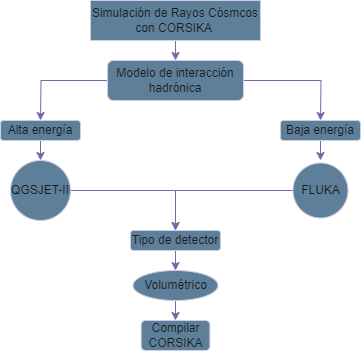
\includegraphics[width=1.25\textwidth]{Figures/methodology_diagram1.png}
                    \includesvg[width=1.2\textwidth]{Figures/methodology_diagram1.svg}
                \end{figure}              
            \end{column}
        \end{columns}
    \end{frame}  


    %------------------------------ SLIDE ---------------------------------------
    \setbeamercolor{itemize item}{fg=orange} % Puedes cambiar el color del triángulo
    % Cambia el símbolo del itemize a un triángulo negro
    \setbeamertemplate{itemize item}{\raisebox{0.2ex}{\scriptsize$\blacktriangleright$}}
    \setbeamercolor{itemize item}{fg=red} % Cambia el color del triángulo a naranja

    \begin{frame}{} % cada entorno frame es una diapositiva
        \justifying % para justificar el texto, siempre al inicio de cada frame
        % Añade espacio para mover el bloque hacia arriba
        % Añade espacio para mover el bloque hacia arriba
        \vspace*{-0.1cm} % Ajusta este valor según sea necesario

        \begin{columns}
            \begin{column}{0.5\textwidth} % Columna izquierda para la lista
                \textcolor{blue}{\textbf{FLUKA:}}
                \begin{itemize}
                    \item Paquete de rutinas que usa el método \emph{Monte Carlo}.
                    \item Permite hacer un análisis del comportamiento de las partículas en la materia.
                    \item Se instala de manera independiente y luego se liga a \emph{CORSIKA}.
                \end{itemize}
            \end{column}

            \begin{column}{0.3\textwidth} % Columna derecha para la imagen
                \begin{figure}
                    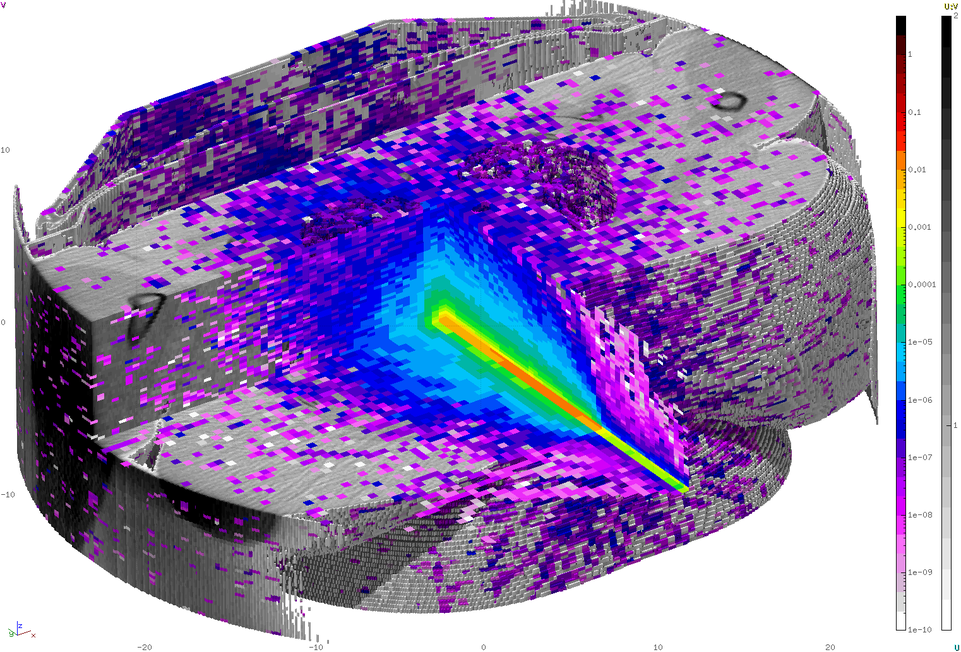
\includegraphics[width=1.2\textwidth]{Figures/fluka.png}
                    \caption{\tiny Visualización de un haz de partículas atravesando un material, realizado con \href{https://fluka.cern/documentation/running/flair-gui}{FLUKA}.}  
                \end{figure}              
            \end{column}
        \end{columns}
    \end{frame}  

    %------------------------------ SLIDE ---------------------------------------
    \setbeamercolor{itemize item}{fg=orange} % Puedes cambiar el color del triángulo
    % Cambia el símbolo del itemize a un triángulo negro
    \setbeamertemplate{itemize item}{\raisebox{0.2ex}{\scriptsize$\blacktriangleright$}}
    \setbeamercolor{itemize item}{fg=red} % Cambia el color del triángulo a naranja

    \begin{frame}{} % cada entorno frame es una diapositiva
        \justifying % para justificar el texto, siempre al inicio de cada frame
        % Añade espacio para mover el bloque hacia arriba
        % Añade espacio para mover el bloque hacia arriba
        \vspace*{-0.2cm} % Ajusta este valor según sea necesario

        \begin{columns}
            \begin{column}{0.5\textwidth} % Columna izquierda para la lista
                \textcolor{blue}{\textbf{Procesamiento de datos y simulaciones:}}
                \begin{itemize}
                    \item Uso del clúster \textbf{LARCAD} (Laboratorio Regional de Cómputo de Alto Desempeño).
                    \item Simulación de millones de cascadas de partículas.
                    \item Espacio de almacenamiento para guardar los resultados de cada simulación. 
                    \item Automatizar procesos mediante scripts para ejecutar CORSIKA en el clúster. 
                \end{itemize}                 
            \end{column}

            \begin{column}{0.3\textwidth} % Columna derecha para la imagen
                \begin{figure}
                    %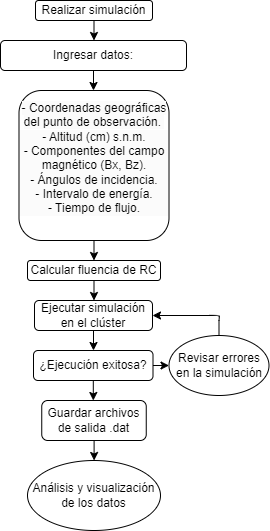
\includegraphics[width=0.8\textwidth]{Figures/methodology_diagram2.png}
                    \includesvg[width=0.85\textwidth]{Figures/methodology_diagram2.svg}
                \end{figure} 
            \end{column}
        \end{columns}
    \end{frame}

    %------------------------------ SLIDE ---------------------------------------
    \setbeamercolor{itemize item}{fg=orange} % Puedes cambiar el color del triángulo
    % Cambia el símbolo del itemize a un triángulo negro
    \setbeamertemplate{itemize item}{\raisebox{0.2ex}{\scriptsize$\blacktriangleright$}}
    \setbeamercolor{itemize item}{fg=red} % Cambia el color del triángulo a naranja

    \begin{frame}{} % cada entorno frame es una diapositiva
        \justifying % para justificar el texto, siempre al inicio de cada frame
        % Añade espacio para mover el bloque hacia arriba
        % Añade espacio para mover el bloque hacia arriba
        \vspace*{-0.4cm} % Ajusta este valor según sea necesario

        \begin{columns}
            \begin{column}{0.7\textwidth} % Columna izquierda para la lista
                \textcolor{blue}{\textbf{Cálculo de la fluencia:}}
                \begin{itemize}
                    \item Rigidez $\mathbf{R_{c}(Lat, Long, Alt, t}, \bm{\theta}, \bm{\phi})$.
                    \item Donde: $\bm{\theta} \in [0^{\circ}, 90^{\circ}]$; $\bm{\phi} \in [0^{\circ}, 360^{\circ}]$.
                    \item Rango de energía para los rayos cósmicos primarios: \\$\mathbf{5 \times 10^{9}}$ \textbf{eV} hasta $\mathbf{10^{15}}$ \textbf{eV}. %\num{5e9} hasta \SI{1e15}{eV}.
                    %\item $N(Z,A,\theta) = \mathcal{N}(\theta) j_{0}(Z,A) \frac{(E/E_{0})^{\alpha ' (Z,A)}}{\alpha ' (Z,A)} \Biggr|_{E_{max}}^{E_{min}}$
                    \item En cada punto de observación se simuló un tiempo, $\mathbf{t = 1}$ hr de flujo.
                    \item Se requirió \textbf{simular} $\mathbf{\sim 450}$  millones de cascadas para 41 puntos de observación.
                \end{itemize}
            \end{column}
            
            \begin{column}{0.3\textwidth} % Columna derecha para la imagen
            \begin{figure}
                    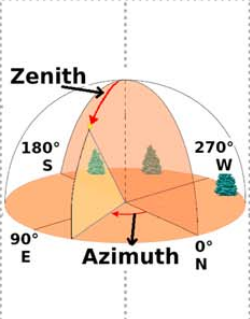
\includegraphics[width=0.5\textwidth]{Figures/angles.png}
                    \caption{\tiny Definición geométrica de los ángulos \textbf{zenital} ($\bm{\theta}$) y \textbf{azimutal} ($\bm{\phi}$) [\cite{asorey2018}].}
            \end{figure}
            \end{column}
        \end{columns}
    \end{frame}

    %------------------------------ SLIDE ---------------------------------------
    %\begin{frame}{} % cada entorno frame es una diapositiva
        %\justifying % para justificar el texto, siempre al inicio de cada frame
        % Añade espacio para mover el bloque hacia arriba
        % Añade espacio para mover el bloque hacia arriba
        %\vspace*{-0.1cm} % Ajusta este valor según sea necesario
        % Cuadro sin bordes redondeados, con colores personalizados
        %\begin{tcolorbox}[colback=custombgcolor9, coltext=customfgcolor2,
            %colframe=custombgcolor9, % Color del borde
            %width=\textwidth,       % Ancho del cuadro
            %boxrule=1pt,            % Grosor del borde
            %top=1mm, bottom=1mm,     % Espacio superior e inferior
            %sharp corners=all,     % Bordes sin redondear
            %halign=center,         % Alineación horizontal
            %valign=center,         % Alineación vertical
                      %]
            % Texto dentro del cuadro
            %\textbf{Diagrama \kern-0.9em de \kern-0.9em Flujo}
        %\end{tcolorbox}  
        
		%\begin{figure}
			%\centering
    		%\begin{minipage}{0.3\textwidth}
				%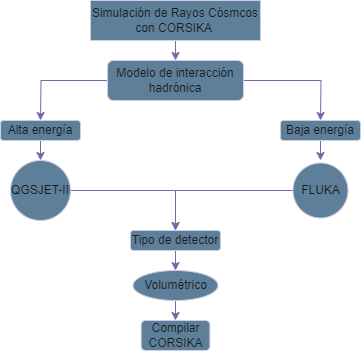
\includegraphics[width=\textwidth]{Figures/methodology_diagram1.png}
			%\end{minipage}
			%\hfill
			%\begin{minipage}{0.2\textwidth}
				%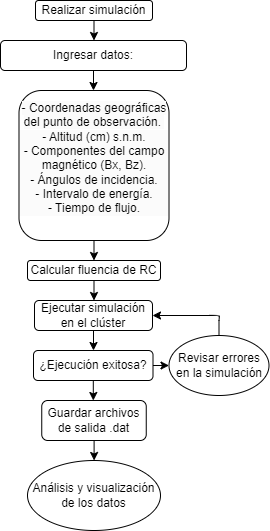
\includegraphics[width=\textwidth]{Figures/methodology_diagram2.png}
			%\end{minipage}				
		%\end{figure}        
    %\end{frame}